\section{Model-to-text transformation}
\label{sec:m2t}

In the following section, we present the \hilecop{} model-to-text
transformation (HM2T) through its formal specification.  The HM2T
generates a \hvhdl{} design out of an SITPN model.  The main idea
behind the implementation of a SITPN model as a \hvhdl{} design lies
on the creation of instances of the place and transition
designs\footnote{Remember that the \texttt{place} and
  \texttt{transition} designs are two pre-defined designs which
  definition in abstract syntax can be found in
  Appendices~\ref{app:place-design} and \ref{app:trans-design}.} that
will act as subcomponents in the behavior of the generated design. To
each place of the input SITPN model will correspond one place design
instance (PDI), and to each transition will correspond one transition
design instance (TDI). These instances will then be connected together
thus reflecting the arc connections of the input SITPN
model. Moreover, the interpretation elements of the SITPN model,
namely the conditions, actions and functions will be implemented by
the input and output ports of the output design. Therefore, there
exists a mapping between the elements of the input SITPN model and
their corresponding version in the generated \hvhdl{} design. This
mapping is captured within a structure called a SITPN-to-\hvhdl{}
binder.  This structure is generated alongside the transformation of
the input SITPN model into a \hvhdl{} design. Its formal definition is
as follows:
\begin{definition}[SITPN-to-\hvhdl{} design binder]
  \label{def:sitpn-to-hvhdl-binder}
  Given a $sitpn\in{}SITPN$ and a \hvhdl{} design $d\in{}design$, a
  SITPN-to-\hvhdl{} binder $\gamma\in{}WM(sitpn,d)$ is a tuple\\
  ${<}PMap,TMap,CMap,AFMap{>}$ where:
  \begin{itemize}
  \item $PMap\in{}P\rightarrow{}\{id_p~|~\mathtt{comp}(id_p,\mathtt{place},g,i,o)\in{}d.beh\}$
  \item $TMap\in{}T\rightarrow{}\{id_t~|~\mathtt{comp}(id_t,\mathtt{transition},g,i,o)\in{}d.beh\}$
  \item $CMap\in\mathcal{C}\rightarrow\{id_c~|~(\mathtt{in}, id_c, \mathtt{bool})\in{}d.ports\}$
  \item $AFMap\in\mathcal{A}\cup\mathcal{F}\rightarrow\{id_{af}~|~(\mathtt{out}, id_{af}, \mathtt{bool})\in{}d.ports\}$
  \end{itemize}
\end{definition}

For a given binder $\gamma$ and an element of an SITPN structure
$e\in{}P\cup{}T\cup\mathcal{C}\cup\mathcal{A}\cup\mathcal{F}$, we
write $\gamma(e)$ where $e$ is looked up in the appropriate
function. For instance, for a given $f\in\mathcal{F}$, $\gamma(f)$ is
a shorthand notation for $AFMap(f)$ where $\gamma={<}\dots,AFMap{>}$.

\bigskip

The formal specification of the HM2T is expressed as a relation
between the inputs of the transformation, namely a SITPN model and a
bounding function, and its outputs, namely a \hvhdl{} design and a
SITPN-to-\hvhdl{} binder. The relation is written
$HM2T_{\mathtt{spec}}\subseteq{}SITPN\times(P\rightarrow\mathbb{N})\times{}design\times{}WM(sitpn,d)$.
The bounding function, that is, the second parameter of the relation,
associates each place of the SITPN model with a bound in terms of
number of tokens.  A bound represents the maximum number of tokens
that a place will possibly hold at some point of the execution of the
model. We assume that these bounds have been computed through the
formal analysis of the input SITPN model. Of course, the existence of
such a function implies that all the SITPN models that are passed as
inputs to the HM2T are \textit{bounded} models\footnote{There exists
  no place that can accumulate an unlimited number of tokens in the
  course of the execution of the model.}. As a matter of fact, we can
prove that the HM2T is not semantic-preserving when the input is an
unbounded SITPN model. The execution of such a model will lead to an
infinite incrementation of the number of tokens in a given place. This
infinite incrementation, while valid in the mathematical world, can
never be mirrored by a \vhdl{} implementation of the model where all
values must be finite. Therefore, the behavior of the SITPN model and
its \hvhdl{} implementation will diverge at a certain point of their
execution.

\bigskip

Definition~\ref{def:hm2t-spec} presents the formal specification of
the HM2T. Here only selected points of the definition are presented
and illustrated. The full definition of the HM2T's formal
specification can be found at \todo{Add ref. to formal
  spec. ref. (Arxiv or equivalent).}. We have implemented the
$HM2T_{\mathtt{spec}}$ relation in \coq{}, and have written a \coq{}
function, named \texttt{sitpn2hvhdl}, that implements the
transformation but is yet to be proved sound and complete regarding
its specification. % However, the
% proof of semantic preservation implies that some properties must be
% drawn regarding the implementation of the HM2T as a program.
% However, all the properties that must be proved to state that the
% HM2T is semantic preserving contribute to the proof of soundness of
% our program w.r.t. its specification.
While expressing the $HM2T_{\mathtt{spec}}$ relation, we refer to sets
and functions that we define below:

\begin{itemize}
\item \texttt{input}$(p)=\{t~\vert~post(t,p)=\lfloor\omega\rfloor\}$,
  the set of input transitions of place $p$.
\item
  \texttt{output}$(p)=\{t~\vert~pre(p,t)=\lfloor(\omega,a)\rfloor\}$,
  the set of output transitions of place $p$.

\item \texttt{acts}$(p)=\{a~\vert~\mathbb{A}(p,a)=\mathtt{true}\}$,
  the set of actions associated with place $p$.
\item
  \texttt{input}$(t)=\{p~\vert~pre(p,t)=\lfloor(\omega,a)\rfloor\}$,
  the set of input places of transition $t$.
\item \texttt{output}$(t)=\{p~\vert~post(t,p)=\lfloor\omega\rfloor\}$,
  the set of output places of transition $t$.
\item
  \texttt{conds}$(t)=\{c~\vert~\mathbb{C}(t,c)=1\lor\mathbb{C}(t,c)=-1\}$,
  the set of conditions associated with transition $t$.
\item
  \texttt{trs}$(c)=\{t~\vert~\mathbb{C}(t,c)=1\lor\mathbb{C}(t,c)=-1\}$,
  the set of transitions with which condition $c$ is associated.
\item \texttt{pls}$(a)=\{p~\vert~\mathbb{A}(p,a)=\mathtt{true}\}$, the
  set of places with which action $a$ is associated.
\item \texttt{trs}$(f)=\{t~\vert~\mathbb{F}(t,f)=\mathtt{true}\}$, the
  set of transitions with which function $f$ is associated.
\end{itemize}

\begin{itemize}
\item \texttt{output}$_c\in{}P\rightarrow{}2^T$.  The
  \texttt{output}$_c$ function takes a place $p$ as input and yields
  an ordered set of transitions computed as follows:
  \begin{enumerate}
  \item If all conflicts between the output transitions of $p$ are
    solved by mutual exclusion, or if the set of conflicting
    transitions of $p$ is a singleton, then \texttt{output}$_c$
    returns an empty set.
  \item Otherwise, the function tries to establish a total ordering
    over the set of conflicting transitions of $p$ w.r.t the firing
    priority relation:
    \begin{itemize}
    \item If no such ordering can be established (in that case, the
      firing priority relation is ill-formed, and the input SITPN is
      not well-defined), \texttt{output}$_c$ raises an error.
    \item Otherwise, the function returns the set in a decreasing
      priority order.
    \end{itemize}
  \end{enumerate}
\end{itemize}

\bigskip

In Definition~\ref{def:hm2t-spec}, we also refer to the names of
generic constants and signals declared in the place and transition
designs. To achieve conciseness, we use aliases to refer to these
constants and signals. The correspondence between the aliases and the
full names is given in Appendix~\ref{sec:cnsts-sigs-names}.

%%%%% Definition for the HM2T formal specification. %%%%%

\def\pdiInBeh{\mathtt{comp}(\gamma(p),\mathtt{place},g_p,i_p,o_p)\in{}d.beh}
\def\tdiInBeh{\mathtt{comp}(\gamma(t),\mathtt{transition},g_t,i_t,o_t)\in{}d.beh}
\def\tdiInBehP#1{\mathtt{comp}(\gamma(#1),\mathtt{transition},g_{#1},i_{#1},o_{#1})\in{}d.beh}

\begin{definition}[\hilecop{} model-to-text transformation specification]
  \label{def:hm2t-spec}
  For all SITPN model $sitpn\in{}SITPN$, bounding function
  $b\in{}P\rightarrow\mathbb{N}$, \hvhdl{} design $d\in{}design$, and
  SITPN-to-\hvhdl{} binder $\gamma\in{}WM(sitpn,d)$, we have
  $HM2T_{\mathtt{spec}}(sitpn,b,d,\gamma)$ if:
  
  \begin{enumerate}
  \item\label{it:emp-gen-clause} Design $d$ has an empty generic clause: $d.gens=\emptyset$.

  \item The number of input ports of the design is equal to the number
    of conditions of the SITPN model:
    $\vert\{id~\vert~(\mathtt{in},id,\tau)\in{}d.ports\}\vert=\vert\mathcal{C}\vert$.
  \item The number of output ports of the design is equal to the
    number of actions and functions of the SITPN model:
    $\vert\{id~\vert~(\mathtt{out},id,\tau)\in{}d.ports\}\vert=\vert\mathcal{A}\cup{}\mathcal{F}\vert$.

  \item\label{it:pdi-tdi-only} All design instantiation statement in
    the design's behavior
    either creates a PDI or a TDI: \\
    $\forall{}id_c,id_e,g,i,o~s.t.~\mathtt{comp}(id_c,id_e,g,i,o)\in{}d.beh,~id_e=\mathtt{place}\lor{}id_e=\mathtt{transition}$.
    
  \item\label{it:actions-functions-only} The \texttt{actions} and
    \texttt{functions} processes are the
    only two processes in the design's behavior:\\
    $\forall{}id_p,vars,ss~s.t.~\mathtt{ps}(id_p,vars,ss)\in{}d.beh,~id_p=\mathtt{actions}\lor{}id_p=\mathtt{functions}$.
    
  \item\label{it:d-is-elaborable} Design $d$ is elaborable in the context of the \hilecop{} design store\footnote{The \hilecop{} design store is a specific design store that holds the definition of the \texttt{place} and \texttt{transition} designs.} and given an empty dimensioning function:\\
    $\exists{}\Delta\in{}ElDesign,\sigma_e\in\Sigma$ s.t.
    $\mathcal{D_\mathcal{H}},\emptyset\vdash{}d\xrightarrow{elab}\Delta,\sigma_e$.
    
  \item\label{it:binder-bij} All the fields of the SITPN-to-\hvhdl{} binder are bijective
    functions: $PMap(\gamma)$ is bijective, $TMap(\gamma)$ is
    bijective,\dots
  \end{enumerate}

  \bigskip
  
  Points~\ref{it:emp-gen-clause} to \ref{it:binder-bij} describe the
  global shape of the output design $d$ and the binder structure
  $\gamma$.  Point~\ref{it:pdi-tdi-only} states that the behavior of
  design d is only composed of place or transition design
  instances. Point~\ref{it:actions-functions-only} states that there
  are only two processes in the behavior of the output design, namely
  the $\mathtt{actions}$ process and the $\mathtt{functions}$
  process. Their content are specified in Points~\ref{it:actions} and
  \ref{it:functions}. Point~\ref{it:d-is-elaborable} states that the
  output design is elaborable, i.e. syntactically well-formed,
  statically well-typed, with no multiply-driven signals, etc.
  Point~\ref{it:binder-bij} states that there is a one-to-one
  correspondence between the elements of the input SITPN model and the
  elements of the output design and that this correspondence is
  established through the binder $\gamma$.

  \bigskip
  
  \begin{enumerate}[resume]
  \item\label{it:pdi-exists} For all place of the input SITPN model,
    there exists a corresponding PDI identified through $\gamma$ in
    the behavior of the output
    design:\\
    $\forall{}p\in{}P,\exists{}g_p,i_p,o_p$ s.t.  $\pdiInBeh$.
    
  \item\label{it:pdi-gmap} For all place of the input SITPN model and
    its corresponding PDI, the generic map of the PDI holds the
    following associations:
    
    \begin{equation*}
      \begin{aligned}
        \forall{}p\in&{}P,g_p,i_p,o_p, \\
        & \pdiInBeh\Rightarrow \\
        &
          \begin{aligned}
            g_p=\{&(\mathtt{mm}\Rightarrow{}b(p)), (\mathtt{ian}\Rightarrow
            \begin{cases}
              1~\mathrm{if}~\mathtt{input}(p)=\emptyset \\
              \vert{}\mathtt{input}(p)\vert~\mathrm{otherwise} \\
            \end{cases}), \\
            &(\mathtt{oan}\Rightarrow
            \begin{cases}
              1~\mathrm{if}~\mathtt{output}(p)=\emptyset \\
              \vert{}\mathtt{output}(p)\vert~\mathrm{otherwise} \\
            \end{cases})\} \\
          \end{aligned}
        \\
      \end{aligned}
    \end{equation*}
    
  \item\label{it:pdi-im} For all place of the input SITPN model and
    its corresponding PDI, there is an association between the
    \texttt{im} input port and the initial marking of the place in the
    input port map of the PDI:\\
    $\forall{}p\in{}P,g_p,i_p,o_p,\pdiInBeh{}$
    $\Rightarrow(\mathtt{im}\Rightarrow{}M_0(p))\in{}i_p$.
  \end{enumerate}

  \bigskip

  Point~\ref{it:pdi-exists} states the existence of a corresponding
  PDI in the behavior of the output design for each place of the input
  SITPN model. Point~\ref{it:pdi-gmap} describes how the content of
  the generic map of a PDI is computed based on the properties of the
  corresponding place. Point~\ref{it:pdi-im} describes how the initial
  marking of place is reflected on the input port map of the
  corresponding PDI through the \texttt{im} input
  port. Figure~\ref{fig:gen-pci-ex} illustrates the link between the
  number of input and output arcs of a place and how this information
  is passed through the generic map and impacts the dimensioning of
  the corresponding PDI's port interface.

  \begin{figure}[h]
    \centering
    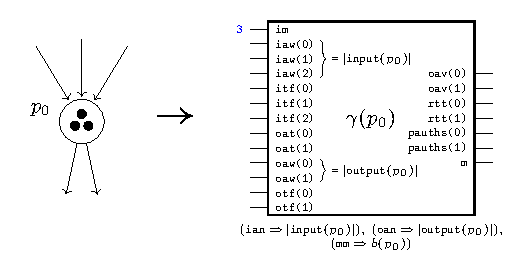
\includegraphics[keepaspectratio,width=.7\textwidth]{gen-pci-ex.eps}
    \caption{A graphical representation of the interface of the PDI
      $\gamma(p_0)$ (on the right) implementing place $p_0$ (on the
      left). The generic map associations appear underneath the PDI.}
    \label{fig:gen-pci-ex}
  \end{figure}
  
  \begin{enumerate}[resume]

  \item\label{it:exists-tdi} For all transition of the input SITPN model, there exists a
    corresponding TDI identified through $\gamma$ in the behavior of
    the output design:\\
    $\forall{}t\in{}T,\exists{}g_t,i_t,o_t$ s.t. $\tdiInBeh$.
    
  \item\label{it:tdi-gen-map} For all transition of the input SITPN model and its
    corresponding TDI, the generic map of the TDI holds the following
    associations:
    \begin{equation*}
      \begin{aligned}[t]
        \forall{}t&\in{}T,g_t,i_t,o_t, \\
                  & \tdiInBeh\Rightarrow \\
                  & g_t=\{(\mathtt{tt}\Rightarrow{}
                    \begin{cases}
                      \mathtt{not\_temp}~\mathrm{if}~t\notin{}\mathtt{dom}(I_s) \\
                      \mathtt{temp\_a\_a}~\mathrm{if}~I_s(t)=[a,a] \\
                      \mathtt{temp\_a\_b}~\mathrm{if}~I_s(t)=[a,b] \\
                      \mathtt{temp\_a\_inf}~\mathrm{if}~I_s(t)=[a,\infty] \\
                    \end{cases}),
        (\mathtt{mtc}\Rightarrow
        \begin{cases}
          1~\mathrm{if}~t\notin{}\mathtt{dom}(I_s) \\
          b~\mathrm{if}~I_s(t)=[a,b] \\
          a~\mathrm{if}~I_s(t)=[a,\infty] \\
        \end{cases}), \\
                  & (\mathtt{ian}\Rightarrow
                    \begin{cases}
                      1~\mathrm{if}~\mathtt{input}(t)=\emptyset \\
                      \vert{}\mathtt{input}(t)\vert~\mathrm{otherwise} \\
                    \end{cases}), 
        (\mathtt{cn}\Rightarrow
        \begin{cases}
          1~\mathrm{if}~\mathtt{conds}(t)=\emptyset \\
          \vert{}\mathtt{conds}(t)\vert~\mathrm{otherwise} \\
        \end{cases})\}. \\
      \end{aligned}
    \end{equation*}
    
  \item\label{it:tdi-time-itval} For all transition of the input SITPN
    model and its corresponding TDI, the input port map of the TDI
    holds the following associations:
    \begin{equation*}
      \begin{aligned}[t]
        \forall{}t&\in{}T,g_t,i_t,o_t, \\
                  & \tdiInBeh\Rightarrow \\
                  & \{(\mathtt{A}\Rightarrow\begin{cases}
                                              0~\mathrm{if}~t\notin\mathtt{dom}(I_s) \\
                                              l(I_s(t))~\mathrm{otherwise} \\
                                            \end{cases}),
        (\mathtt{B}\Rightarrow\begin{cases}
                                0~\mathrm{if}~t\notin\mathtt{dom}(I_s)\lor{}u(I_s(t))=\infty \\
                                u(I_s(t))~\mathrm{otherwise} \\
                              \end{cases})\}\subseteq{}i_t. \\
      \end{aligned}
    \end{equation*}

  \end{enumerate}

  \bigskip

  Similarly to the case of places, Points~\ref{it:exists-tdi} to
  \ref{it:tdi-time-itval} state the existence of a corresponding TDI
  for each transition of the input model, and how its generic map and
  its input port map are built regarding the properties of the
  transition, namely: the shape of the time interval, the number of
  input arcs, the number of associated conditions,
  etc. Figure~\ref{fig:gen-tdi-ex} illustrates the relation between
  the properties of a transition and how they are implemented in the
  interface of the corresponding TDI.

  \begin{figure}[h]
    \centering
    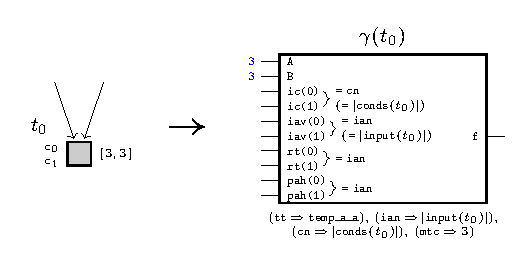
\includegraphics[keepaspectratio,width=.8\textwidth]{gen-tdi-ex.eps}
    \caption{A graphical representation of the interface of the TDI
      $\gamma(t_0)$ (on the right) implementing transition $t_0$ (on
      the left). The generic map associations appear underneath the
      TDI.}
    \label{fig:gen-tdi-ex}
  \end{figure}
  
  \begin{enumerate}[resume]        
  \item\label{it:post-arc} For all post arc of the input SITPN model,
    the TDI and PDI corresponding to the source transition and target
    place of the arc are connected as follows:
    \begin{equation*}
      \begin{aligned}[t]
        \forall{}t&\in{}T,p\in{}P,g_t,i_t,o_t,g_p,i_p,o_p,\omega\in\mathbb{N}^{*}, \\
                  & post(t,p)=\lfloor\omega\rfloor\Rightarrow \\
                  & \tdiInBeh\Rightarrow \\
                  & \pdiInBeh\Rightarrow\\
                  & \exists{}i\in[0,\vert\mathtt{input}(p)\vert-1]~s.t.~(\mathtt{iaw}(i)\Rightarrow\omega)\in{}i_p \\
                  & \land\exists{}id_s~s.t.~(id_s,\mathtt{bool})\in{}d.sigs
                    \land(\mathtt{fired}\Rightarrow{}id_s)\in{}o_t\land(\mathtt{itf}(i)\Rightarrow{}id_s)\in{}i_p. \\
      \end{aligned}
    \end{equation*}

  \end{enumerate}
  
  \bigskip

  Figure~\ref{fig:gen-post-arc} illustrates the translation of a post
  arc of the input SITPN model as described in
  Point~\ref{it:post-arc}. The weight of the arc is passed to the PDI
  through the \texttt{iaw} input port. In the behavior of the output
  design, all arc information is encoded through the input port
  interface of PDIs. All computations that necessitate the arc
  information, such as the marking update or the setting of time
  counter reset signals, are performed in the behavior of the place
  design. Therefore, only the PDIs need to hold the arc information.

  \begin{figure}[h]
    \centering
    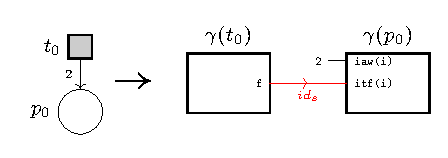
\includegraphics[keepaspectratio,width=.7\textwidth]{gen-post-arc.eps}
    \caption{The translation of a post arc connecting a transition
      $t_0$ to a place $p_0$ into an interconnection between the
      interfaces of the corresponding TDI and PDI.}
    \label{fig:gen-post-arc}
  \end{figure}
  
  \begin{enumerate}[resume]
  \item\label{it:pre-arc} For all pre arc of the input SITPN model,
    the PDI and TDI corresponding to the source place and target
    transition of the arc are connected as follows:
    \begin{equation*}
      \begin{aligned}[t]
        \forall{}t&\in{}T,p\in{}P,g_t,i_t,o_t,g_p,i_p,o_p,\omega\in\mathbb{N}^{*},a\in\{\mathtt{basic},\mathtt{test},\mathtt{inhib}\}, \\
                  & pre(p,t)=\lfloor(\omega,a)\rfloor\Rightarrow \\
                  & \tdiInBeh\Rightarrow \\
                  & \pdiInBeh\Rightarrow\\
                  & \exists{}i\in[0,\vert\mathtt{output}(p)\vert-1]~s.t.~\{(\mathtt{oaw}(i)\Rightarrow\omega),(\mathtt{oat}(i)\Rightarrow{}a)\}\subseteq{}i_p \\
                  & \begin{aligned}[t]
                      \land\exists{}j &\in[0,\vert\mathtt{input}(t)\vert-1],id_{av},id_{rt},id_{frd},id_{pah}~s.t. \\
                                      & \{(id_{av},\mathtt{bool}),(id_{rt},\mathtt{bool}),(id_{frd},\mathtt{bool}),(id_{pah},\mathtt{bool})\}\subseteq{}d.sigs \\
                                      & \land(\mathtt{oav}(i)\Rightarrow{}id_{av})\in{}o_p\land(\mathtt{iav}(j)\Rightarrow{}id_{av})\in{}i_t \\
                                      & \land(\mathtt{rtt}(i)\Rightarrow{}id_{rt})\in{}o_p\land(\mathtt{rt}(j)\Rightarrow{}id_{rt})\in{}i_t \\
                                      & \land(\mathtt{otf}(i)\Rightarrow{}id_{frd})\in{}i_p\land(\mathtt{fired}\Rightarrow{}id_{frd})\in{}o_t \\
                                      & \land(\mathtt{pah}(i)\Rightarrow{}id_{frd})\in{}o_p \\
                                      & \land(a=\mathtt{test}\lor{}a=\mathtt{inhib}\lor{}\mathtt{output}_c(p)=\emptyset\Rightarrow(\mathtt{pah}(j)\Rightarrow\mathtt{true})\in{}i_t) \\
                                      & \land(a=\mathtt{basic}\land{}\mathtt{output}_c(p)\neq\emptyset\Rightarrow(\mathtt{pah}(j)\Rightarrow{}id_{pah})\in{}i_t). \\
                    \end{aligned} \\
      \end{aligned}
    \end{equation*}
  \end{enumerate}

  \bigskip
  
  Figure~\ref{fig:gen-pre-arc} illustrates the translation of a pre
  arc of the input SITPN model as described in Point~\ref{it:pre-arc}.
  Here, we assume that there remain some conflicts not solved by
  mutual exclusion in the set of output transitions of place
  $p_0$. Otherwise, according to Point~\ref{it:pre-arc}, the
  interconnection between $\mathtt{pah(i)}$ and $\mathtt{pah(j)}$
  would not be effective.
  
  \begin{figure}[h]
    \centering
    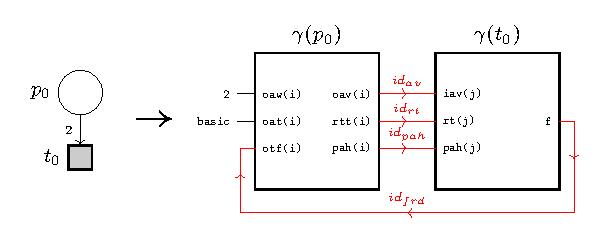
\includegraphics[keepaspectratio,width=.8\textwidth]{gen-pre-arc.eps}
    \caption{The translation of a pre arc, connecting a place $p_0$ to
      a transition $t_0$, into an interconnection between the
      interfaces of the corresponding PDI and TDI. }
    \label{fig:gen-pre-arc}
  \end{figure}

  \begin{enumerate}[resume]
  \item\label{it:port-indices-ordering} For all place of the input
    SITPN model for which conflicts in its output transitions are not
    solved by mutual exclusion, the port indices of the corresponding
    PDI reflect the priority order established between the conflicting
    output transitions:
    \begin{equation*}
      \begin{aligned}[t]
        \forall{}p&\in{}P,t,t'\in{}\mathtt{output}_c(p),g_p,i_p,o_p,g_t,i_t,o_t,g_{t'},i_{t'},o_{t'}, \\
                  & t\succ{}t'\Rightarrow\\
                  & \pdiInBeh\Rightarrow \\
                  & \tdiInBehP{t}\Rightarrow \\
                  & \tdiInBehP{t'}\Rightarrow \\
                  &
                    \begin{aligned}[t]
                      (\forall{}i,j&\in\mathbb{N},id_{frd},id_{frd'}, \\
                                   & (\mathtt{fired}\Rightarrow{}id_{frd})\in{}o_t\Rightarrow \\
                                   & (\mathtt{fired}\Rightarrow{}id_{frd'})\in{}o_{t'}\Rightarrow \\
                                   & \{(\mathtt{otf}(i)\Rightarrow{}id_{frd}),(\mathtt{otf}(j)\Rightarrow{}id_{frd'})\}\subseteq{}i_p\Rightarrow \\
                                   & i<j) \\
                    \end{aligned} \\
                  & \begin{aligned}[t]
                      \land(\forall{}i,j&\in\mathbb{N},id_{s},id_{s'},name_t,name_{t'},id_{pout}, \\
                                        & (name_t\Rightarrow{}id_{s})\in{}i_t\Rightarrow \\
                                        & (name_{t'}\Rightarrow{}id_{s'})\in{}i_{t'}\Rightarrow \\
                                        & \{(id_{pout}(i)\Rightarrow{}id_s),(id_{pout}(j)\Rightarrow{}id_{s'})\}\subseteq{}o_p\Rightarrow \\
                                        & i<j). \\
                    \end{aligned} \\
      \end{aligned}
    \end{equation*}
  \end{enumerate}

  \bigskip

  Figure illustrates the ordering of the port indices in the interface
  of PDIS as described in Point~\ref{it:port-indices-ordering}.

  \begin{figure}[h]
    \centering
    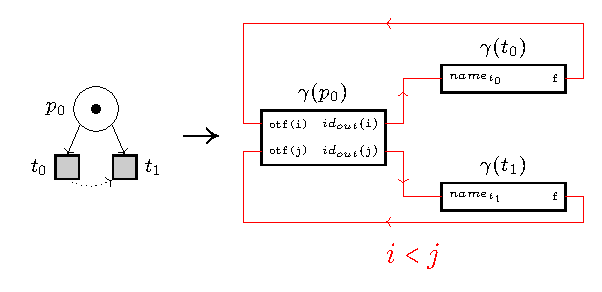
\includegraphics[keepaspectratio,width=.8\textwidth]{gen-prio-order.eps}
    \caption{Translation of the priority relation in terms of port
      index ordering. Here, $name_{t_0}$ (resp. $name_{t_1}$) refers
      to any input port of TDI $\gamma(t_0)$ (resp. $\gamma(t_1)$),
      and $id_{out}$ refers to any composite output port of PDI
      $\gamma(p_0)$.}
    \label{fig:gen-prio-order}
  \end{figure}

  \begin{enumerate}[resume]
  \item\label{it:actions} There exists an \texttt{actions} process
    that assigns a value to the output port representing the
    activation status of the actions (referred to as \textit{action}
    ports) of the input SITPN model:
    
    $\exists{}ss_{ra},ss_{a}~s.t.~\mathtt{ps}(\mathtt{actions},\emptyset,\mathtt{rst}\{ss_{ra}\}\mathtt{else}\{\mathtt{falling}\{ss_a\}\})\in{}d.beh$
    and
    \begin{enumerate}
    \item The length of the $ss_{ra}$ and $ss_{a}$ sequences is equal
      to the number of actions of the input SITPN model:\\
      $\vert{}ss_{ra}\vert_{;}=\vert{}ss_a\vert_{;}=\vert\mathcal{A}\vert$ where $\vert{}ss\vert{}_{;}=
      \begin{cases}
        \vert{}ss_1\vert_{;}+\vert{}ss_2\vert_{;}~\mathrm{if}~ss=ss_1;ss_2 \\
        1~\mathrm{otherwise}
      \end{cases}
      $
    \item During the initialization, all action ports are assigned to
      \texttt{false} by the \texttt{actions} process:\\
      $\forall{}a\in\mathcal{A},~\gamma(a)\Leftarrow\mathtt{false}\in{}ss_{ra}$
    \item An action port corresponding to an action associated with no
      place is assigned to \texttt{false} during the falling edge
      phase:\\
      $\forall{}a\in\mathcal{A}~s.t.~\mathtt{pls}(a)=\emptyset,\gamma(a)\Leftarrow\mathtt{false}\in{}ss_{a}$
      
    \item Otherwise, the value of the action port is the result of the
      Boolean sum between the \texttt{marked} output port of all PDIs
      representing the places associated with the considered action:
      \begin{equation*}
        \begin{aligned}[t]
          \forall{}a\in\mathcal{A},&~\mathtt{pls}(a)\neq\emptyset\Rightarrow \\
                                   &\exists{}e_{or}~s.t.~\gamma(a)\Leftarrow{}e_{or}\in{}ss_a\land\mathtt{is\_bsum}(e_{or},\vert{}\mathtt{pls}(a)\vert) \\
                                   &
                                     \begin{aligned}[t]
                                       \land\forall{}p\in{}& \mathtt{pls}(a),g_p,i_p,o_p,\\
                                                           & \pdiInBeh\Rightarrow \\
                                                           & \exists{}id_m~s.t.~(id_m,\mathtt{bool})\in{}d.sigs\land{}id_m\in{}e_{or}\land(\mathtt{marked}\Rightarrow{}id_m)\in{}o_p\\
                                     \end{aligned} \\
        \end{aligned}
      \end{equation*}
      where $\mathtt{is\_bsum}$ is defined as follows:

      \vspace{10pt}
      
      \begin{tabular}{l}
        {\begin{prooftree}
            \hypo{e\in{}\{id,b\}}
            \infer1{\mathtt{is\_bsum}(e,1)}
          \end{prooftree}} \\
      \end{tabular}
      \begin{tabular}{l}
        {\begin{prooftree}
            \hypo{\mathtt{is\_bsum}(e_1,n)}
            \hypo{\mathtt{is\_bsum}(e_2,m)}
            \infer2
            {\mathtt{is\_bsum}(\mathtt{or}(e_1,e_2),n+m)}
          \end{prooftree}} \\
      \end{tabular}
      
    \end{enumerate}

    % \item\label{it:functions} There exists an \texttt{functions}
    %   process that assigns a value to the output port representing the
    %   execution status of the functions (referred to as
    %   \textit{function} ports) of the input SITPN model:
    
    %   $\exists{}ss_{rf},ss_{f}~s.t.~\mathtt{ps}(\mathtt{functions},\emptyset,\mathtt{rst}\{ss_{rf}\}\mathtt{else}\{\mathtt{rising}\{ss_f\}\})\in{}d.beh$
    %   and
    % \begin{enumerate}
    % \item The length of the $ss_{rf}$ and $ss_{f}$ sequences is equal
    %   to the number of functions of the input SITPN model:\\
    %   $\vert{}ss_{rf}\vert_{;}=\vert{}ss_f\vert_{;}=\vert\mathcal{F}\vert$
      
    % \item During the initialization, all function ports are assigned
    %   to
    %   \texttt{false} by the \texttt{functions} process:\\
    %   $\forall{}f\in\mathcal{F},~\gamma(f)\Leftarrow\mathtt{false}\in{}ss_{rf}$
      
    % \item A function port that implements a function associated with
    %   no transition is assigned to \texttt{false} during the rising
    %   edge
    %   phase:\\
    %   $\forall{}f\in\mathcal{F}~s.t.~\mathtt{trs}(f)=\emptyset,\gamma(f)\Leftarrow\mathtt{false}\in{}ss_{f}$
      
    % \item Otherwise, the value of the function port is the result of
    %   the Boolean sum between the \texttt{fired} output port of all
    %   TDIs representing the transitions associated with the
    %   corresponding function:
    %   \begin{equation*}
    %     \begin{aligned}[t]
    %       \forall{}f\in\mathcal{F},&~\mathtt{trs}(f)\neq\emptyset\Rightarrow \\
    %                                &\exists{}e_{or}~s.t.~\gamma(f)\Leftarrow{}e_{or}\in{}ss_f\land\mathtt{is\_bsum}(e_{or},\vert{}\mathtt{trs}(f)\vert) \\
    %                                &
    %                               \begin{aligned}[t]
    %                                 \land\forall{}t\in{}& \mathtt{trs}(f),g_t,i_t,o_t,\\
    %                                                     & \tdiInBeh\Rightarrow \\
    %                                                     & \exists{}id_m~s.t.~(id_m,\mathtt{bool})\in{}d.sigs\land{}id_m\in{}e_{or}\land(\mathtt{fired}\Rightarrow{}id_m)\in{}o_t \\
    %                               \end{aligned} \\
    %     \end{aligned}
    %   \end{equation*}      
    % \end{enumerate}
    
  \item For all association between a transition and a condition, the
    input port reflecting the Boolean value of the given condition
    (referred to as a \textit{condition} port) is connected as follows
    to the input port map of the TDI corresponding to the associated
    transition:
    \begin{equation*}
      \begin{aligned}[t]
        \forall{}t&\in{}T,g_t,i_t,o_t,c\in\mathcal{C}, \\
                  & \tdiInBeh\Rightarrow \\
                  & (\mathbb{C}(t,c)=1\Rightarrow\exists{}i\in[0,\vert\mathtt{conds}(t)\vert-1]~s.t.~(\mathtt{ic}(i)\Rightarrow{}\gamma(c))\in{}i_t) \\
                  & (\mathbb{C}(t,c)=-1\Rightarrow\exists{}i\in[0,\vert\mathtt{conds}(t)\vert-1]~s.t.~(\mathtt{ic}(i)\Rightarrow{}\mathtt{not}(\gamma(c)))\in{}i_t). \\
      \end{aligned}
    \end{equation*}
    

  \end{enumerate}

\end{definition}

%%% Local Variables:
%%% mode: latex
%%% TeX-master: "main"
%%% End:
